\chapter{Create your own objects}
\label{chap09}

\section{Class definitions and object types}
\label{classes}
\index{type!object}
\index{type!user-defined}
\index{object type}
\index{class definition}
\index{user-defined type}

% Every time you write a class definition, you create a new
% object type with the same name as the class.
Way back in
Section~\ref{hello} when we defined the class {\tt Hello},
we also created an object type named {\tt Hello}.  We
didn't create any variables with type {\tt Hello}, and we
didn't use {\tt new} to create any {\tt Hello}
objects, but we could have!

That example doesn't make much sense, since there is no
reason to create a {\tt Hello} object, and it wouldn't do
much if we did.  In this chapter, we
will look at class definitions that create
{\em useful} object types.

Here are the most important ideas in this chapter:

\begin{itemize}

\item Defining a new class also creates a new object type
with the same name.

\item A class definition is like a template for objects:
it determines what instance variables the objects have and
what methods can operate on them.

\item Every object belongs to some object type; that is, it
is an instance of some class.

\item When you invoke {\tt new} to create an object, Java
invokes a special method called a {\bf constructor} to initialize the
instance variables.  You provide one or more constructors as part of
the class definition.

\item The methods that operate on a type are defined in the
class definition for that type.

\end{itemize}

Here are some syntax issues about class definitions:

\begin{itemize}

\item Class names (and hence object types) should begin with a capital
letter, which helps distinguish them from primitive types and variable
names.

\item You usually put one class definition in each file, and the name
of the file must be the same as the name of the class, with the suffix
{\tt .java}.  For example, the {\tt Time} class is defined in the file
named {\tt Time.java}.

\item In any program, one class is designated as the {\bf startup
class}.  The startup class must contain a method named {\tt main}, which
is where the execution of the program begins.  Other classes {\em may}
have a method named {\tt main}, but it will not be executed.

\end{itemize}

With those issues out of the way, let's look at an example of
a user-defined class, {\tt Time}.


\section{Time}
\index{class!Time}
\index{Time}

A common motivation for creating an object type is to encapsulate
related data in an object that can be treated as a single unit.  We
have already seen two types like this, {\tt Point} and {\tt
Rectangle}.

Another example, which we will implement ourselves, is {\tt Time},
which represents the time of day.  The data encapsulated in a Time
object are an hour, a minute, and a number of seconds.  Because every
{\tt Time} object contains these data, we need instance
variables to hold them.

The first step is to decide what type each variable should be.  It
seems clear that {\tt hour} and {\tt minute} should be integers.  Just
to keep things interesting, let's make {\tt second} a {\tt double}.

\index{instance variable}
\index{variable!instance}

Instance variables are declared at the beginning of the class
definition, outside of any method definition, like this:

\begin{lstlisting}
class Time {
    int hour, minute;
    double second;
}
\end{lstlisting}
%
By itself, this code fragment is a legal class definition.  The
state diagram for a {\tt Time} object looks like this:


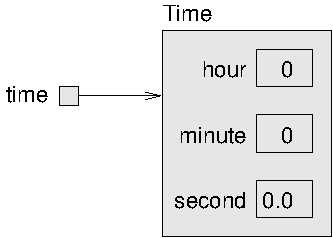
\includegraphics{figs/time.pdf}


After declaring the instance variables, the next step is
to define a constructor for the new class.

\section{Constructors}
\index{constructor}
\index{method!constructor}
\index{static}

Constructors initialize instance
variables.  The syntax for constructors is similar to that
of other methods, with three exceptions:

\begin{itemize}

\item The name of the constructor is the same as the name of
the class.

\item Constructors have no return type and no return value.

\item The keyword {\tt static} is omitted.

\end{itemize}

Here is an example for the {\tt Time} class:

\begin{lstlisting}
    public Time() {
        this.hour = 0;
        this.minute = 0;
        this.second = 0.0;
    }
\end{lstlisting}
%
Where you would expect to see a return type,
between {\tt public} and {\tt Time}, there is nothing.  That's
how we (and the compiler) can tell that this is a constructor.

This constructor does not take any arguments.  Each line of the
constructor initializes an instance variable to a default
value (in this case, midnight).  The name {\tt this} is a special
keyword that refers to the object we are creating.  You can use
{\tt this} the same way you use the name of any other object.  For
example, you can read and write the instance variables of {\tt this},
and you can pass {\tt this} as an argument to other methods.

\index{this}

But you do not declare {\tt this} and you can't make an
assignment to it.  {\tt this} is created by the system; all you
have to do is initialize its instance variables.

A common error when writing constructors is to put a {\tt return}
statement at the end.  Resist the temptation.


\section{More constructors}
\index{overloading}

Constructors can be overloaded, just like other methods,
which means that you can provide multiple constructors
with different parameters.  Java knows which constructor
to invoke by matching the arguments of {\tt new}
with the parameters of the constructors.

It is common to have one constructor that takes no
arguments (shown above), and one constructor that takes
a parameter list identical to the list of instance
variables.  For example:

\begin{lstlisting}
    public Time(int hour, int minute, double second) {
        this.hour = hour;
        this.minute = minute;
        this.second = second;
    }
\end{lstlisting}
%
The names and types of the parameters are the same as
the names and types of the instance variables.  All the
constructor does is copy the information from the parameters
to the instance variables.

If you look at the documentation for {\tt Point}s
and {\tt Rectangle}s, you will see that both classes provide
constructors like this.  Overloading constructors provides the
flexibility to create an object first and then fill in the
blanks, or to collect all the information before creating
the object.

This might not seem very interesting, and in fact it
is not.  Writing constructors is a boring, mechanical process.
Once you have written two, you will find that you can write them
quickly just by looking at the list of instance
variables.


\section{Creating a new object}
\index{new}
\index{statement!new}

Although constructors look like methods, you never invoke them
directly.  Instead, when you invoke {\tt new}, the system
allocates space for the new object and then
invokes your constructor.

The following program demonstrates two ways to create and
initialize {\tt Time} objects:

\begin{lstlisting}
class Time {
    int hour, minute;
    double second;

    public Time() {
        this.hour = 0;
        this.minute = 0;
        this.second = 0.0;
    }

    public Time(int hour, int minute, double second) {
        this.hour = hour;
        this.minute = minute;
        this.second = second;
    }

    public static void main(String[] args) {

        // one way to create and initialize a Time object
        Time t1 = new Time();
        t1.hour = 11;
        t1.minute = 8;
        t1.second = 3.14159;
        System.out.println(t1);

        // another way to do the same thing
        Time t2 = new Time(11, 8, 3.14159);
        System.out.println(t2);
    }
}
\end{lstlisting}
%
In {\tt main}, the first time we invoke {\tt new},
we provide no arguments, so Java invokes the first constructor.
The next few lines assign values to the instance
variables.

The second time we invoke {\tt new}, we provide
arguments that match the parameters of the second constructor.
This way of initializing the instance variables is more concise
and slightly more efficient, but it can be harder to read, since
it is not as clear which values are assigned to which instance
variables.


\section{Printing objects}
\label{printobject}
\index{print}
\index{statement!print}
\index{object!printing}

The output of this program is:

\begin{verbatimtab}
Time@80cc7c0
Time@80cc807
\end{verbatimtab}
%
When Java prints the value of a user-defined object type, it prints
the name of the type and a special hexadecimal (base 16) code that is
unique for each object.  This code is not meaningful in itself; in
fact, it can vary from machine to machine and even from run to run.
But it can be useful for debugging, in case you want to keep track of
individual objects.

To print objects in a way that is more meaningful to users
(as opposed to programmers), you can write a method
called something like {\tt printTime}:

\begin{lstlisting}
    public static void printTime(Time t) {
        System.out.println(t.hour + ":" + t.minute + ":" + t.second);
    }
\end{lstlisting}
%
Compare this method to the version of {\tt printTime} in
Section~\ref{time}.

The output of this method, if we pass either {\tt t1} or {\tt t2} as
an argument, is {\tt 11:8:3.14159}.  Although this is recognizable
as a time, it is not quite in the standard format.  For example, if
the number of minutes or seconds is less than 10, we expect a leading
{\tt 0} as a place-keeper.  Also, we might want to drop the decimal
part of the seconds.  In other words, we want something like
{\tt 11:08:03}.

In most languages, there are simple ways to control the output format
for numbers.  In Java there are no simple ways.

Java provides powerful tools for printing formatted things
like times and dates, and also for interpreting formatted input.
Unfortunately, these tools are not very easy to use, so I am going to
leave them out of this book.  If you want, you can take a look
at the documentation for the {\tt Date} class in the {\tt
java.util} package.
\index{Date}
\index{class!Date}


\section{Operations on objects}
\label{objectops}
\index{object}
\index{operator!object}

In the next few
sections, I demonstrate three kinds of methods that
operate on objects:

\begin{description}

\item[pure function:]  Takes objects as
arguments but does not modify them.  The return value is
either a primitive or a new object created inside the method.

\item[modifier:]  Takes objects as arguments and modifies some
or all of them.  Often returns void. \index{void}

\item[fill-in method:]  One of the arguments is an ``empty''
object that gets filled in by the method.  Technically, this is
a type of modifier.

\end{description}

Often it is possible to write a given method as a pure function, a modifier,
or a fill-in method.  I will discuss the pros and cons of each.


\section{Pure functions}
\index{pure function}
\index{function}
\index{method!pure function}

A method is considered a pure function if the result depends only on
the arguments, and it has no side effects like modifying an argument
or printing something.  The only result of invoking a pure function is
the return value.

One example is {\tt isAfter}, which compares two {\tt Time}s and
returns a {\tt boolean} that indicates whether the first operand
comes after the second:

\begin{lstlisting}
    public static boolean isAfter(Time time1, Time time2) {
        if (time1.hour > time2.hour) return true;
        if (time1.hour < time2.hour) return false;

        if (time1.minute > time2.minute) return true;
        if (time1.minute < time2.minute) return false;

        if (time1.second > time2.second) return true;
        return false;
    }
\end{lstlisting}
%
What is the result of this method if the two times are equal?  Does
that seem like the appropriate result for this method?  If you were
writing the documentation for this method, would you mention that case
specifically?

A second example is {\tt addTime}, which calculates the sum of two
times.  For example, if it is {\tt 9:14:30}, and your breadmaker takes
3 hours and 35 minutes, you could use {\tt addTime} to figure out when
the bread will be done.

Here is a rough draft of this method that is not quite right:

\begin{lstlisting}
    public static Time addTime(Time t1, Time t2) {
        Time sum = new Time();
        sum.hour = t1.hour + t2.hour;
        sum.minute = t1.minute + t2.minute;
        sum.second = t1.second + t2.second;
        return sum;
    }
\end{lstlisting}
%
Although this method returns a {\tt Time} object, it is not
a constructor.  You should go back and compare the syntax of
a method like this with the syntax of a constructor, because
it is easy to get confused.

Here is an example of how to use this method.  If {\tt currentTime}
contains the current time and {\tt breadTime} contains the amount
of time it takes for your breadmaker to make bread, then you
could use {\tt addTime} to figure out when the bread will be
done.

\begin{lstlisting}
    Time currentTime = new Time(9, 14, 30.0);
    Time breadTime = new Time(3, 35, 0.0);
    Time doneTime = addTime(currentTime, breadTime);
    printTime(doneTime);
\end{lstlisting}
%
The output of this program is {\tt 12:49:30.0}, which is
correct.  On the other hand, there are cases where the result
is not correct.  Can you think of one?

The problem is that this method does not deal with cases
where the number of seconds or minutes adds up to more than
60.  In that case, we have to ``carry'' the extra seconds
into the minutes column, or extra minutes into the hours
column.

Here's a corrected version of the method.

\begin{lstlisting}
    public static Time addTime(Time t1, Time t2) {
        Time sum = new Time();
        sum.hour = t1.hour + t2.hour;
        sum.minute = t1.minute + t2.minute;
        sum.second = t1.second + t2.second;

        if (sum.second >= 60.0) {
            sum.second -= 60.0;
            sum.minute += 1;
        }
        if (sum.minute >= 60) {
            sum.minute -= 60;
            sum.hour += 1;
        }
        return sum;
    }
\end{lstlisting}
%
Although it's correct, it's starting to get big.  Later
I suggest much shorter alternative.

\index{increment}
\index{decrement}
\index{operator!increment}
\index{operator!decrement}

This code demonstrates two operators we have not seen before,
{\tt +=} and {\tt -=}.  These operators provide a concise
way to increment and decrement variables.  They are similar
to {\tt ++} and {\tt --}, except (1) they work on {\tt double}s
as well as {\tt int}s, and (2) the amount of the increment
does not have to be 1.  The statement {\tt sum.second -= 60.0;}
is equivalent to {\tt sum.second = sum.second - 60;}


\section{Modifiers}
\index{modifier}
\index{method!modifier}

As an example of a modifier, consider {\tt increment},
which adds a given number of seconds to a {\tt Time} object.
Again, a rough draft of this method looks like:

\begin{lstlisting}
    public static void increment(Time time, double secs) {
        time.second += secs;

        if (time.second >= 60.0) {
            time.second -= 60.0;
            time.minute += 1;
        }
        if (time.minute >= 60) {
            time.minute -= 60;
            time.hour += 1;
        }
    }
\end{lstlisting}
%
The first line performs the basic operation; the remainder
deals with the same cases we saw before.

Is this method correct?  What happens if the argument {\tt secs}
is much greater than 60?  In that case, it is not enough to
subtract 60 once; we have to keep doing it until {\tt second}
is below 60.  We can do that by replacing the {\tt if}
statements with {\tt while} statements:

\begin{lstlisting}
    public static void increment(Time time, double secs) {
        time.second += secs;

        while (time.second >= 60.0) {
            time.second -= 60.0;
            time.minute += 1;
        }
        while (time.minute >= 60) {
            time.minute -= 60;
            time.hour += 1;
        }
    }
\end{lstlisting}
%
This solution is correct, but not very efficient.
Can you think of a solution that does not require iteration?


\section{Fill-in methods}
\index{fill-in method}
\index{method!fill-in}

Instead of creating a new object every time {\tt addTime} is
invoked, we could require the caller to provide an
object where {\tt addTime} stores the result.  Compare
this to the previous version:

\begin{lstlisting}
    public static void addTimeFill(Time t1, Time t2, Time sum) {
        sum.hour = t1.hour + t2.hour;
        sum.minute = t1.minute + t2.minute;
        sum.second = t1.second + t2.second;

        if (sum.second >= 60.0) {
            sum.second -= 60.0;
            sum.minute += 1;
        }
        if (sum.minute >= 60) {
            sum.minute -= 60;
            sum.hour += 1;
        }
    }
\end{lstlisting}
%
The result is stored in {\tt sum}, so the return type is {\tt void}.

Modifiers and fill-in methods are efficient because they
don't have to create new objects.  But they make it more
difficult to isolate parts of a program; in large projects they can
cause errors that are hard to find.

Pure functions help manage the complexity of large projects,
in part by making certain kinds of errors impossible.  Also, they
lend themselves to certain kids of composition and nesting.
And because the result of a pure function depends only on the parameters,
it is possible to speed them up by storing previously-computed
results.
\index{pure function}

I recommend that you write pure functions whenever
it is reasonable, and resort to modifiers only if there
is a compelling advantage.


\section{Incremental development and planning}
\index{incremental development}
\index{prototyping}
\index{program development!incremental}
\index{program development!planning}

In this chapter I demonstrated a program development process called
{\bf rapid prototyping}\footnote{What I am calling rapid prototyping
  is similar to test-driven development (TDD); the difference is that
  TDD is usually based on automated testing.  See
  \url{http://en.wikipedia.org/wiki/Test-driven_development}.}.  For
each method, I wrote a rough draft that performed the
basic calculation, then tested it on a few cases, correcting flaws
as I found them.

This approach can be effective, but it can lead to code
that is unnecessarily complicated---since it deals with many
special cases---and unreliable---since it is hard to convince
yourself that you have found {\em all} the errors.

An alternative is to look for insight
into the problem that can make the programming easier.  In
this case the insight is that a {\tt Time} is really a three-digit
number in base 60!  The {\tt second} is the ``ones column,''
the {\tt minute} is the ``60's column'', and the {\tt hour}
is the ``3600's column.''

When we wrote {\tt addTime} and {\tt increment}, we were effectively
doing addition in base 60, which is why we had to ``carry'' from one
column to the next.

\index{arithmetic!floating-point}

Another approach to the whole problem is to convert
{\tt Time}s into {\tt double}s and take advantage of the fact that
the computer already knows how to do arithmetic with {\tt double}s.
Here is a method that converts a {\tt Time} into a {\tt double}:

\begin{lstlisting}
        public static double convertToSeconds(Time t) {
        int minutes = t.hour * 60 + t.minute;
        double seconds = minutes * 60 + t.second;
        return seconds;
    }
\end{lstlisting}
%
Now all we need is a way to convert from a {\tt double}
to a {\tt Time} object.  We could write a method to
do it, but it might make more sense to write it as a third
constructor:

\begin{lstlisting}
    public Time(double secs) {
        this.hour =(int)(secs / 3600.0);
        secs -= this.hour * 3600.0;
        this.minute =(int)(secs / 60.0);
        secs -= this.minute * 60;
        this.second = secs;
    }
\end{lstlisting}
%
This constructor is a little different from the others;
it involves some calculation along with assignments to the
instance variables.

You might have to think to convince yourself that the technique
I am using to convert from one base to another is correct.  But once
you're convinced, we can use these methods to rewrite {\tt addTime}:

\begin{lstlisting}
    public static Time addTime(Time t1, Time t2) {
        double seconds = convertToSeconds(t1) + convertToSeconds(t2);
        return new Time(seconds);
    }
\end{lstlisting}
%
This is shorter than the original version, and it is much easier
to demonstrate that it is correct (assuming, as usual, that the
methods it invokes are correct).  As an exercise, rewrite {\tt
increment} the same way.


\section{Generalization}
\index{generalization}

In some ways converting from base 60 to base 10 and back is
harder than just dealing with times.  Base conversion is more
abstract; our intuition for dealing with times is better.

But if we have the insight to treat times as base 60 numbers,
and make the investment of writing the conversion methods
({\tt convertToSeconds} and the third constructor), we get
a program that is shorter, easier to read and debug, and more
reliable.

It is also easier to add features later.  Imagine
subtracting two {\tt Time}s to find the duration between them.  The
naive approach would be to implement subtraction complete with
``borrowing.''  Using the conversion methods would be much easier.

Ironically, sometimes making a problem harder (more general)
makes it easier (fewer special cases, fewer opportunities for error).


\section{Algorithms}
\label{algorithm}
\index{algorithm}

When you write a general solution for a class of problems, as
opposed to a specific solution to a single problem, you have
written an {\bf algorithm}.  This word is
not easy to define, so I will try a couple of approaches.

First, consider some things that are not algorithms.  When you learned
to multiply single-digit numbers, you probably memorized the
multiplication table.  In effect, you memorized 100 specific
solutions, so that knowledge is not really algorithmic.

But if you were ``lazy,'' you probably learned a few
tricks.  For example, to find the product of $n$ and 9, you can
write $n-1$ as the first digit and $10-n$ as the second digit.  This
trick is a general solution for multiplying any single-digit number by 9.
That's an algorithm!

Similarly, the techniques you learned for addition with carrying,
subtraction with borrowing, and long division are all algorithms.  One
of the characteristics of algorithms is that they do not require any
intelligence to carry out.  They are mechanical processes in which
each step follows from the last according to a simple set of rules.

In my opinion, it is embarrassing that humans spend so much
time in school learning to execute algorithms that,
quite literally, require no intelligence.
%
On the other hand, the process of designing algorithms is
interesting, intellectually challenging, and a central part
of what we call programming.

Some of the things that people do naturally, without difficulty
or conscious thought, are the most difficult to express
algorithmically.  Understanding natural language is a good
example.  We all do it, but so far no one has been able to
explain {\em how} we do it, at least not in the form of an
algorithm.

Soon you will have the opportunity to design
simple algorithms for a variety of problems.


\section{Glossary}

\begin{description}

\item[class:]  Previously, I defined a class as a collection
of related methods.  In this chapter we learned that a class
definition is also a template for a new type of object.

\item[instance:]  A member of a class.  Every object is an
instance of some class.

\item[constructor:]  A special method that initializes the instance
variables of a newly-constructed object.

\item[startup class:]  The class that contains the {\tt main}
method where execution of the program begins.

\item[pure function:]  A method whose result depends only on its
parameters, and that has no side-effects other than returning
a value.

\item[modifier:]  A method that changes one or more of the objects
it receives as parameters, and usually returns {\tt void}.

\item[fill-in method:]  A type of method that takes an ``empty''
object as a parameter and fills in its instance variables instead
of generating a return value.

\item[algorithm:]  A set of instructions for solving a class of
problems by a mechanical process.

\index{class}
\index{instance}
\index{constructor}
\index{startup class}
\index{pure function}
\index{modifier}
\index{algorithm}

\end{description}


\section{Exercises}

\begin{exercise}
In the board game Scrabble\footnote{Scrabble is a registered trademark
owned in the U.S.A and Canada by Hasbro Inc., and in the rest of the world
by J.W. Spear \& Sons Limited of Maidenhead, Berkshire, England, a subsidiary
of Mattel Inc.}, each tile contains a letter, which is used to spell
words, and a score, which is used to determine the value of words.

\begin{enumerate}

\item Write a definition for a class named {\tt Tile}
that represents Scrabble tiles.  The instance variables should
be a character named {\tt letter} and an integer named {\tt value}.

\item Write a constructor that takes parameters named {\tt letter}
and {\tt value} and initializes the instance variables.

\item Write a method named {\tt printTile} that takes a {\tt Tile}
object as a parameter and prints the instance variables in
a reader-friendly format.

\item Write a method named {\tt testTile} that creates a
Tile object with the letter {\tt Z} and the value 10, and
then uses {\tt printTile} to print the state of the object.

\end{enumerate}

The point of this exercise is to practice the mechanical part
of creating a new class definition and code that tests it.
\end{exercise}


\begin{exercise}
Write a class definition for {\tt Date}, an object type that
contains three integers, {\tt year}, {\tt month} and {\tt day}.
This class should provide two constructors.  The first should
take no parameters.  The second should take parameters named
{\tt year}, {\tt month} and {\tt day}, and use them to initialize
the instance variables.

Write a {\tt main} method that creates a new {\tt Date} object
named {\tt birthday}.  The new object should contain your birthdate.
You can use either constructor.
\end{exercise}


\begin{exercise}
\label{ex.rational}

A rational number is a number that can be represented as the ratio of
two integers.  For example, $2/3$ is a rational number, and you can
think of 7 as a rational number with an implicit 1 in the denominator.
For this assignment, you are going to write a class definition for
rational numbers.

\begin{enumerate}

\item Create a new program called {\tt Rational.java} that defines a
class named {\tt Rational}.  A {\tt Rational} object should have two
integer instance variables to store the numerator and denominator.

\item Write a constructor that takes no arguments and that sets the
numerator to 0 and denominator to 1.

\item Write a method called {\tt printRational} that takes
a Rational object as an argument and prints it in some
reasonable format.

\item Write a {\tt main} method that creates a new object with
type Rational, sets its instance variables to some values, and prints
the object.

\item At this stage, you have a minimal testable
program.  Test it and, if necessary, debug it.

\item Write a second constructor for your class that takes two
arguments and that uses them to initalize the instance
variables.

\item Write a method called {\tt negate} that reverses the sign of
a rational number.  This method should be a modifier, so it should
return {\tt void}.  Add lines to {\tt main} to test the new method.

\item Write a method called {\tt invert} that inverts the number by
  swapping the numerator and denominator.  Add lines to {\tt main} to
  test the new method.

\item Write a method called {\tt toDouble} that converts the rational
number to a double (floating-point number) and returns the result.
This method is a pure function; it does not modify the object.
As always, test the new method.

\item Write a modifier named {\tt reduce} that reduces a rational
  number to its lowest terms by finding the greatest common divisor
  (GCD) of the numerator and denominator and dividing through.
  This method should be a pure function; it should
  not modify the instance variables of the object on which it is
  invoked.  To find the GCD, see Exercise~\ref{gcd}).

\item Write a method called {\tt add} that takes two Rational
numbers as arguments and returns a new Rational object.  The return
object should contain the sum of the arguments.

There are several ways to add fractions.  You can use any one you
want, but you should make sure that the result of the operation is
reduced so that the numerator and denominator have no common divisor
(other than 1).
\end{enumerate}

The purpose of this exercise is to write a class definition that
includes a variety of methods, including constructors, modifiers and
pure functions.
\end{exercise}




